%
% File: chap04.tex
% Author: ta16969
%
\let\textcircled=\pgftextcircled
\chapter{Program Overview and Evaluation}
\label{chap:Overview and Evaluation}







\initial{T}he purpose of the chapter is to briefly identify Artemis\textquotesingle s features and explain the results of User Evaluation Testing on the aforementioned. The results will be critically analyzed to explain how the code has been re factored due to User Testing and Evaluation. 


\section{Artemis Features}

The key features of Artemis are listed and briefly explained as follows:

\begin{enumerate}

    \item Log In and Registration: As illustrated in Figure \textbf{\ref{ariaHidden}} the application is accessed via a standard registration or log-in page that uses dynamically generated forms. Given that form \& erroneous data validation accessibility, as well as other aspects such as sensitive data encryption have been thoroughly explained, this feature should not require elaboration.
    
    \item Live Search: As illustrated in Figure \textbf{ \ref{ariaHidden}} the application contains a live search feature in the Artemis UI via the header element. Search results are generated by constant AJAX calls to query  MariaDB, so as to create results that reflect each user input/key stroke. The SQL queries use the expression to sub-string pattern recognition  feature of MariaDB i.e. the \textit{LIKE} condition. Each individual search result is  based on the following order of query attributes:
        \begin{enumerate}
            \item Expression patterns that match username.
            \item Expression patterns that match first \textbf{and} last name.
            \item Expression patterns that match either first \textbf{or} last name.
        \end{enumerate}
        
    Should neither of these conditions yield a result, no search results will be returned.
    

    \item Scrolling Newsfeed and Personal Wall: Users can scroll to the bottom of their newsfeed or personal wall to dynamically generate content, public posts for the former and personal ones for the latter. This has been implemented via AJAX calls to query MariaDB, to dynamically generate HTML elements; triggered by a script that simply compares between scrollHeight and inner div height (simple jQuery methods). Note that this method seems compatible with most browser quirks (some browsers seem to add single arbitrary pixel to HTML element heights; creating a host of cross compatibility issues).
    
    \item Messaging System: Artemis has a personal messaging system that can always be accessed via the navigation bar or alternatively the user's personal profile. From a conceptually abstract perspective the logic for generating messages is almost identical to that of creating news feed posts via AJAX calls; except for different formatting for the messages and DB logic to implement access control or privacy. However there is also subtle difference. The messages table in MariaDB contains two attributes independent off the posts attributes i.e. opened and viewed. These attributes indicate whether a message has been viewed from the navigation bar and/or opened and read; allowing for resultant formatting options if desired as illustrated below. These attributes could be useful for implementing advanced messaging features in the future, such as message read receipts.
    
    \begin{figure}[H]
        \begin{center}
            \subfloat{ 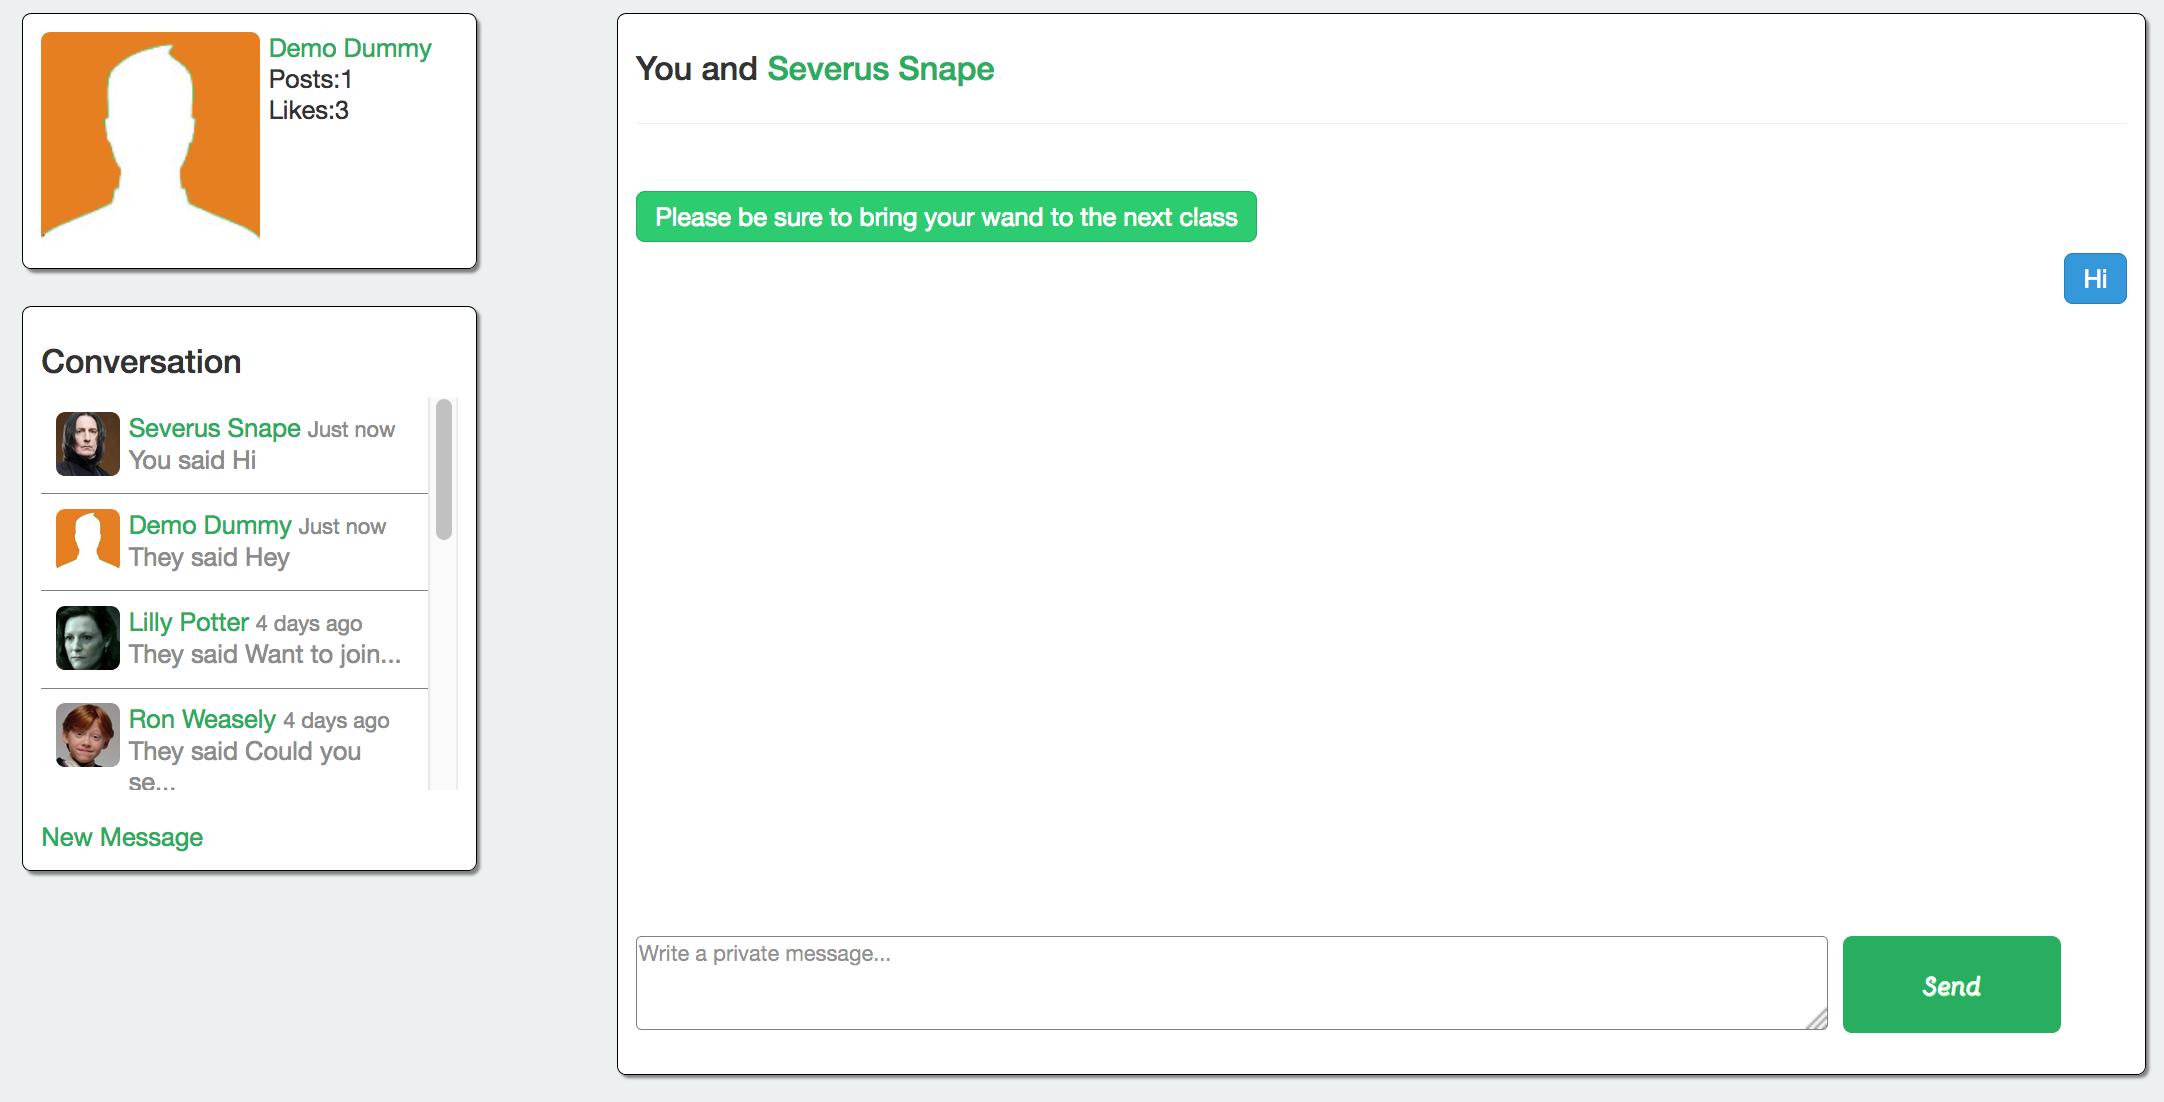
\includegraphics[scale=0.23]{chapters/chapter04/figures/messageDetails.png}}
            \subfloat{ 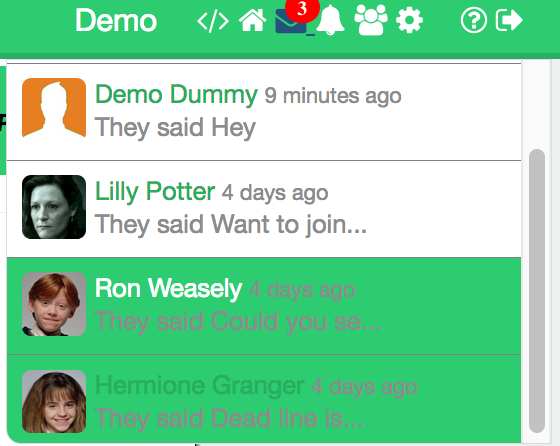
\includegraphics[scale=0.57]{chapters/chapter04/figures/messageNotifications.png}}
            \caption[Snapshot of Artemis Messaging System]{Snapshot of Artemis Messaging System}
            \label{messagingSystem}
        \end{center}
    \end{figure}
        
   
    \item Likes, Posts and  Message Notifications: As indicated earlier messages and posts are database entities with corresponding attributes that can be used for notifications. Notification and Likes are themselves DB entities with their s own attributes. To illustrate the internal DB schema for Artemis the following Entity Relationship (ER) model (crows foot notation) has been provided as per Figure \ref{ERmodel}.
    
    The ER model depicts the relationships of the entities, complexities such as cardinalities and participation, as well as the attributes of the entities. The resultant data base logic and relationships has be queried to count the number of relevant unread messages, unread notifications and friend requests to notify the user as illustrated in Figures \textbf{\ref{dropDown} } \& \textbf{\ref{messagingSystem}}. Certain  attributes of DB entities such as the \textit{openend} attribute for the messages entity  results in conditional formatting at an object level, to highlight the importance of the relevant HTML entity. It must be noted that the ER model is an arbitrary one and whilst sufficient for the purposes of this project, should ideally be updated and the code re-factored to reflect a \textbf{normalized} database; work outside the scope of this project.
    
    

    \begin{figure}[h]
    	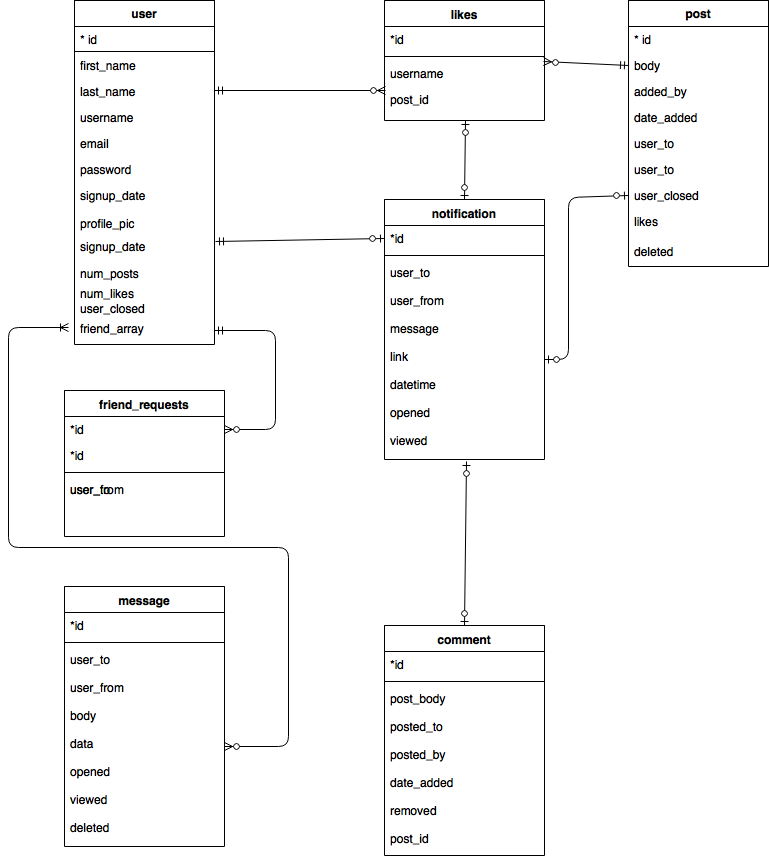
\includegraphics[scale=0.40,center]{chapters/chapter04/figures/crowsFoot.png}
    	\mycaption[ Artemis ER Model ]{Artemis ER Model}
    	\label{ERmodel}
    \end{figure}

    
    \item Settings: Artemis have a access to a user settings page so that they can effectively update their User entity DB attributes; passwords, first/last name, profile picture and deactivate an account. The notable features on this page include the implementation of a form ReCaptcha via the Google api to prevent CSRF attacks on password attributes, an option upload profile pictures for cropping and the use of accessible design features for form validation. As all of these features have been independently discussed in great detail, they do not require further elaboration.
    
    \item Developer Documentation and OER License: As explained on Page \textbf{\pageref{wiki}} as part of the Artemis project, a significant amount of developer documentation aimed at people with technical and non-technical backgrounds alike have been developed to supplement the underlying rationale for making a \textit{Web Credible} solution, not mutually exclusive from good practice with Open Source Projects.  The details of the developer documentation does not require further elaboration (see \pageref{developer}); Except for the legal modality of the project.
    
    The legal modality of the project i.e. the license under which it is disseminated, is relevant because the project was envisioned as an OER \cite{UNESCO}. The MIT license \cite{Github} has been opted for out of a wide range of possible and valid modalities. The reason being that it was short, simple to understand, permissive to the extent desired for an OER \cite{UNESCO} and absolved the author off any resultant liability \cite{Github}. The contents of the license can be found at \url{https://github.com/TaimurAhmed/summerProject2017/wiki/Legal} .
    
    
    
    
\end{enumerate}


\section{User Evaluation and Testing}

    As part of user evaluation and testing for Artemis a sample size of 10 students from the UoB CS department were sought and subjected to series of open ended use cases (Appendix \textbf{\ref{fig:2/6}} ) so that participants may experience all of Artemis features in a limited time period for the purposes of user evaluation and testing. The underlying aim of the use cases was to test Artemis throughly for bugs, undesirable UX features and evaluate whether the UI was Web Credible i.e. to make the aesthetic design \textit{persuasive} against as per the STPL criterion.
    
    The underlying rationale of the questions asked can be broken down as follows:
    \begin{enumerate}
        \item Question 1-12 relate directly to the list of use cases users performed (See page \pageref{fig:2/6}), i.e. to encourage participants to thoroughly test and evaluate \textbf{all} the features of Artemis within the limited time period. As noted earlier users belonging to the CS department at the UoB were asked to try and thoroughly explore the solution beyond the suggested use cases and even attempt to maliciously break it if possible. This approach seems to have resulted in several bugs being detected via the use of unusual or unexplored use cases e.g. the \textit{search bug} illustrated in figure \textbf{\ref{listOBugs}} which was detected by entering gibberish in the search bar.
        
        \item Questions 13 specifically asks for student participants opinions about whether they would prefer to use a social network or the existing TEL solution at UoB, advocated by the TELED team i.e. a forum. The goal here is to gauge interest amongst UoB CS students in the TEL solution before it is deployed.
        
        \item Question 14 onwards relate directly to the underlying design rationale of trying to make the technology persuasive via a Web Credible UI; modelled on the STPL's guidelines on best practice \cite{Fogg2002} e.g. Are users able to contact the developer or people behind the project easily ?
    \end{enumerate}

    The results of user testing are identified and illustrated as follows (See Appendix \textbf{\ref{fig:1/6}} for context):
    
    
    
    \begin{figure}[h]
    	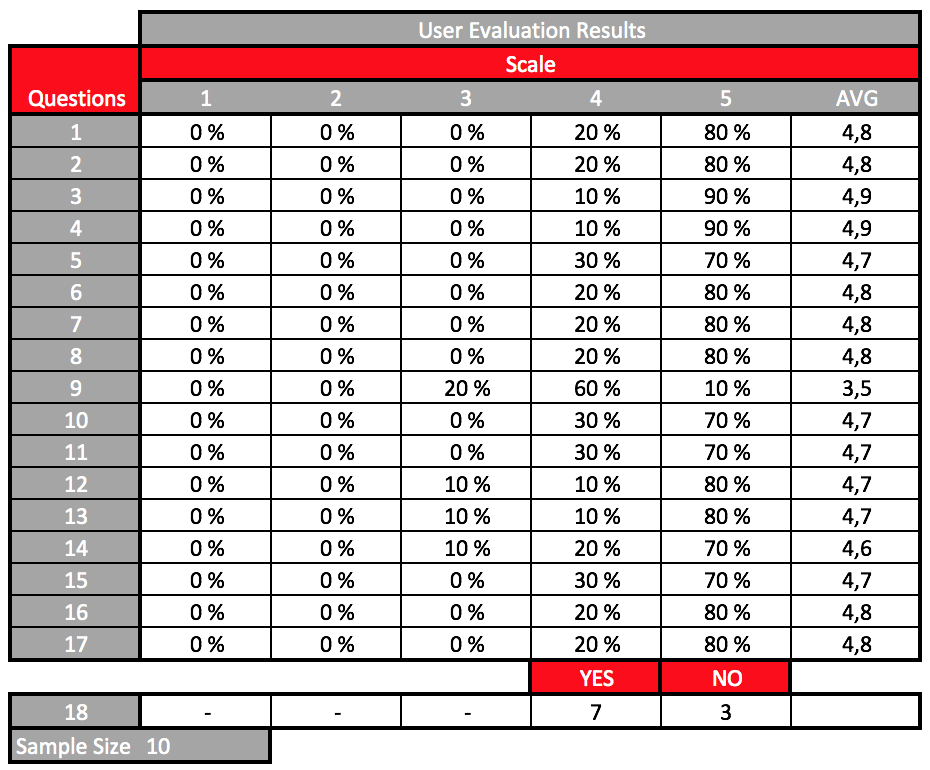
\includegraphics[scale=0.66,center]{chapters/chapter04/figures/userEvaluationTable.png}
    	\mycaption[User Evaluation Results]{User Evaluation Results}
    \end{figure}
    
    \begin{figure}[h]
    	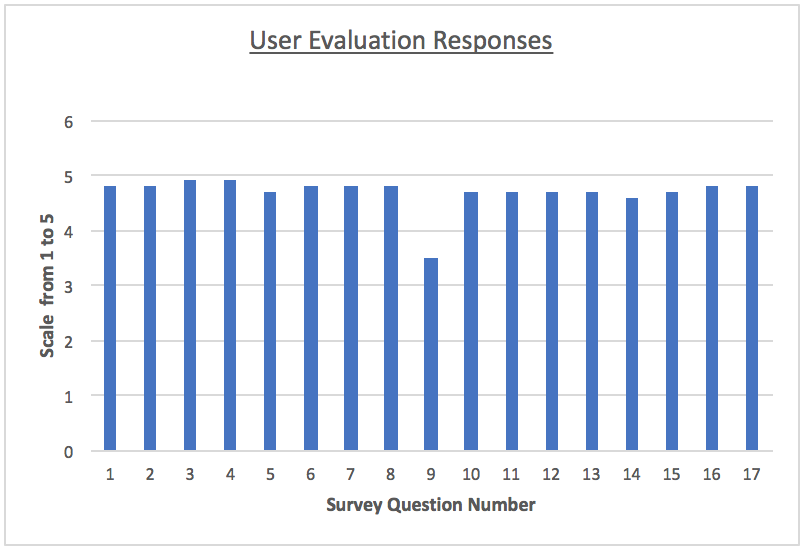
\includegraphics[scale=0.66,center]{chapters/chapter04/figures/userEvaluationGraph.png}
    	\mycaption[User Evaluation Results - Bar Graph]{User Evaluation Results - Bar Graph}
    \end{figure}
    
    
    
    Overall within the scope of this survey, Artemis seems to have scored well with an average score of 4.7 out of 5 as per user feedback. The strategy of letting participants go above and beyond the specified use cases resulted in a list of bugs and user feedback for consideration, as evidenced by 70 percent of the participants discovering some kind of bug or generating feedback as depicted in Figure \textbf{\ref{listOBugs}}. STPL recommends rectifying bugs regardless of impact as they hurt user perception of Web Credibility \cite{Fogg2002}, so all user feedback has been addressed by updating the code accordingly.
    
    The bugs addressed in the source code are elaborated upon as follows (illustrated in Figure \textbf{\ref{listOBugs}}):
    \begin{enumerate}
    
        \item Search Bug: This bug caused segmentation errors due to trying to access unallocated cells of an array, when there were no corresponding results for user input e.g. due to trying to enter gibberish in the search bar. The bug was rectified by preventing access to the relevant array when there were no search results.
        
        \item Aly Bug: This bug caused the logged in User's meta data to appear on the a profile's \textit{section}, as opposed to the owner\textquotesingle s meta data. The bug was caused due to human error i.e. using incorrect variables and subsequently corrected.
        
        \item New Line Bug: This bug was caused when user\textquotesingle s tried to create posts or comments with line breaks. This caused MacOS specific new line carriages to be stored in the database and then subsequently rendered with visible return carriages as opposed to line breaks. To rectify the issue comment and post bodies are now generated with HTML break tags that replace the new line carriages.
        
        \item Form Validation: Certain form error messages were not generated due to incorrect registration credentials, caused by human error during development. The issue was technically simple and easily rectified.
    
    \end{enumerate}
    
    It seems that most users were satisfied with the features provided in Artemis with an average score above 4.7 out of 5. It can be deduced given the scope of the question asked that the users were satisfied with Artemis\textquotesingle s. The exception was Q 9 which resulted in above average but unusually high  feedback i.e. user's wanted to be able to hover over icons and links, to understand their purpose; without needing to click on them. Whilst some users found the icons intuitive and familiar, others struggled at first i.e. validating user feedback that merely choosing familiar icons is not sufficient for everyone. To rectify this a note of the issue was made (See Figure \textbf{\ref{listOBugs}}) and the code re-factored to add previously missing \textit{title attributes} to relevant HTML elements. Adding this feature to the code enables users to hover over UI elements and understand the purpose, without having to click on them.
    
    
    
    
    
    
    
    
    
    
    
    \begin{figure}[h]
    	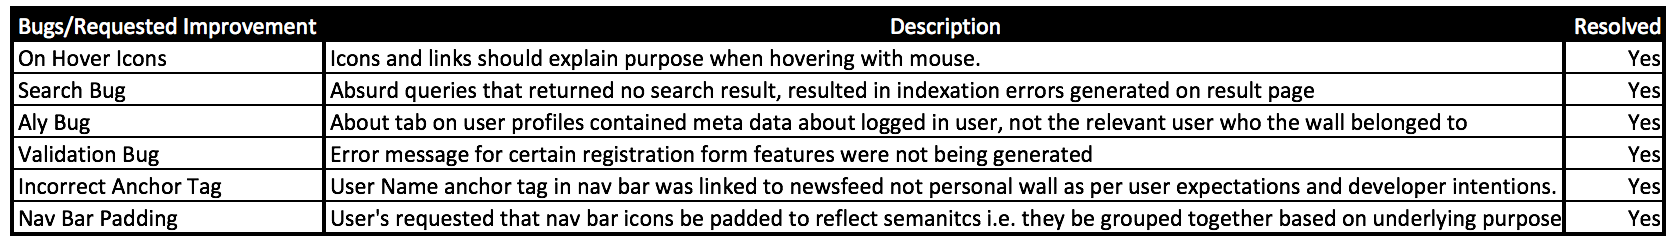
\includegraphics[scale=0.55]{chapters/chapter04/figures/issuesResolved.png}
    	\mycaption[List of User Generated Feedback and Bugs to Refactor Code]{List of User Generated Feedback and Bugs to Refactor Code}
    	\label{listOBugs}
    \end{figure}